\section{Theoretische Rahmenbedinungen}

\subsection{Aktueller Forschungsstand}

\subsubsection{Definitionen}

Zunächst die Definitionen einiger Begrifflichkeiten, welche im Rahmen der Arbeit wiederholt aufgegriffen werden.\newline

\textbf{Refugees - Geflüchtete}

\begin{quote}
    \textit{Refugees are people fleeing conflict or persecution. They are defined and protected in international law, and must not be expelled or returned to situations where their life and freedom are at risk.}\cite{unhcr2017refugees}
\end{quote}
\caption{Definition der UNHCR}

Gemäß der Definition der Vereinten Nationen ist unter einem Geflüchteten jede Person zu verstehen, welche vor Konflikt oder Verfolgung flieht. Sie steht unter dem Schutz des internationalen Rechts und darf nicht in eine Situation entlassen werden, in der Leben oder Freiheit nicht gesichert sind.\newline

refugee:
Firstly, the key word in the UN convention is “persecution”
but it has no single definition. Persecutions can be for
various reasons as defined by the host country and the
scope of persecutions for each host country keeps
expanding and evolving with time. Secondly, there are
numerous routes of arrival into the host country integration
systems. This is alongside the earlier highlighted categories
of persons in the integration system. Refugee integration is
indeed a complicated phenomenon, a situational
information behaviour approach is the only chance that all
the variables in the complexity will be factored into the
understanding.


\textbf{Asylum seekers - Asylsuchende}

\begin{quote}
    \textit{An asylum-seeker is someone whose request for sanctuary has yet to be processed.}\cite{unhcr2015asylum}
\end{quote}
\caption{Definition der UNHCR}

Ein Asylsuchender ist eine Person, deren Antrag auf Asyl in einem Land noch nicht fertig bearbeitet wurde.

At the end of 2017, there were approximately 3.1 million people people around the world waiting for a decision on their asylum claims. For more information and the latest statistics, read our annual Asylum Trends report.

\textbf{Migrants - Migranten}

\begin{quote}
    \textit{Migrants choose to move not because of a direct threat of persecution or death, but mainly to improve their lives by finding work, or in some cases for education, family reunion, or other reasons. Unlike refugees who cannot safely return home, migrants face no such impediment to return. If they choose to return home, they will continue to receive the protection of their government.}\cite{unhcr2016migrant}
\end{quote}
\caption{Definition der UNHCR}

Ein Migrant zieht nicht aufgrund Verfolgung oder Lebensgefahr weiter, sondern um eine verbesserung der Lebensbedingungen zu erreichen. Anders als Geflüchtete, deren Sicherheit am Herkunftsort nicht gewährleistet ist, genießt ein Migrant weiter den Schutz des Herkunftsstaates.


\textbf{Immigrants - Immigranten}

\begin{quote}
    \textit{X}
\end{quote}
\caption{X}  

\textbf{Integration}


Oduntan
The UN convention is operated in an asylum system in
which refugees arrive under different elements. The
systems incorporate varied levels of access to provisions
including support, benefits, work entitlements and rights to
remain. Thus refugee integration starts on arrival in the host
country through the transition process.


\textbf{Informationslücke}

Information Gap:
\cite{dervin2003sense}
sense-making incorporates a repertoire of potenteial procedures for accomplishing the goals discussed preciously. All these are drawn from a xenral metaphor, shown in Figure 12.2 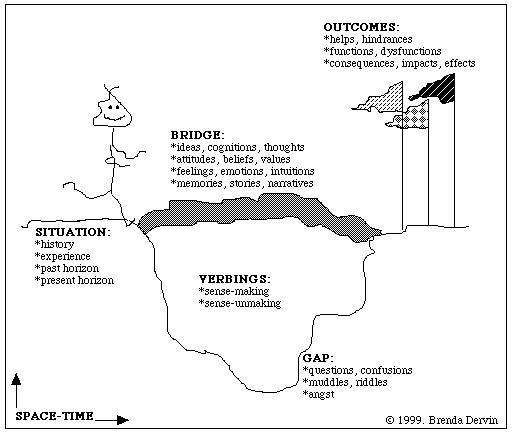
\includegraphics[width=00.5]{SMM_MEtaphor.jpg}. Here, one sees a human moving across time and space, facing a gap, building a bridge across the gap, and then constructing and evaluating the uses of the bridge. This metaphor rests on a descontinuity assumption - that gappiness is pervasive both in and between moments in time and space and in and between people. Gappiness is assumed to occur because of differences across time (e.g. self today vs self yesterday and scientific fact today vs. scientific fact tomorrow) and across space (e.g. the experiece of a particular condition on different cultures, contexts, communites, material circumstances and the sense of an experience physically and the articulation of it verbally)
continue on Dervin p.238


\subsubsection{Stand der Literatur}

Oduntan und Ruthven stellten 2017 im Informationsprozess von Gefl\"uchteten im Asylauswahlverfahrensprozess des Vereinigten K\"onigreichs informationsl\"ucken fest. \cite{oduntan2017investigating}
Mittels semi-strukturierter Interviews nach Dervin's Sense-making Methodology\cite{dervin2003sense} erfolgte eine Zusammenstellung verschiedener Situationen, in denen diese im Rahmen der Studie aufgedeckt wurden - mit dem Hinweis auf die Existenz noch unergr\"undeter Situationen in der Gefl\"uchtetenintegration.\newline
Informationsl\"ucken treten gem\"a\ss{} Derwin aufgrund Abweichungen in Zeit (Ich heute vs. Ich gestern) und Raum (Erfahrung aus dem Blickwinkel verschiedener Kulturen, Werte etc.) auf.\cite{dervin2003sense}\newline
Das Ziel dieser Arbeit ist es, Informationslücken im Integrationsprozess in Deutschland zu identifizieren und untersuchen.\newline
Die Untersuchung fand im Jahr 2019 statt, in der Folgezeit der sogenannten Fl\"uchtlingskrise, welche Europa ab 2015 direkt betraf. \cite{unhcr2015seven}\newline
Hierzu wurde das Informationsverhalten von Gefl\"uchteten untersucht, um Informationsbed\"urfnisse in der deutschen Fl\"uchtlingsintegration festzustellen.\newline
In der Literatur wurden bereits zahlreiche Informationsbedürfnisse und Informationslücken offengelegt\cite{oduntan2017investigating}:
Die Informationsbedürfnisse von Migranten in Queens, NY, wurden von Fisher et al. in Sozialen, Kulturellen und Fähigkeitsbasierten Informationsbedürfnissen kategorisiert. \cite{fisher2004information}
Courtright identifizierte des weiteren medizinische Betreuung, Bildung, Wohnen und Berufstätigkeit bei Lateinamerikanischen Immigranten in Indiana, US. \cite{courtright2005health}
Silvio untersuchte südsudanesische Immigranten in Ontario, US; Ihre Informationsbedürnisse waren auf Bildung, medizinische Betreuung, Berufstätigkeit und politische Informationen bezogen, und suchten nach Mitteln und Wegen, angebracht mit Rassismus umzugehen.\cite{hakim2006information}\newline
Lloyd\cite{lloyd2014building} und Lloyd et al.\cite{lloyd2013connecting}'s Arbeit sind spezifisch auf Geflüchtete und Asylsuchende fokussiert. Lloyd ermittelte Informationsbedürfnisse im Gesundheitssektor, und Lloyd et al. entdeckte Informationsbedürfnisse im Alltag und der Anpassung an soziale Normen; beide Arbeiten beschäftigten sich mit Mündigkeit im Umgang mit Informationen.\newline
All diese Arbeiten sind Personenzentriert; es wird mit relativ kleinen Populationen gearbeitet, bei denen die Informationsbedürfnisse der Individuen untersucht werden. Ausgehend von diesen festgestellten Informationsbedürfnissen kann die Perspektive auf eine größere Population erweitert werden. So können Zusammenhänge zwischen allgemeinem menschlichem Informationsverhalten (\textit{Human Information Behaviour}) und für Geflüchtete und Asylsuchende spezifische Informationsfaktoren herstellt werden.\cite{oduntan2017investigating}\newline
Dies ist insofern wichtig, da etwa Chatman feststellte, dass sich das Informationsverhalten von Randgruppen oft signifikant von dem der Bev\"olkerungsmehrheit unterscheidet. \cite{chatman1996impoverished}
\newline
\newline 
%ICT's
Um den Integrationsprozess zu erleichtern, gab es mehrere Projekte, mit sogenannten ICT's (Information and communications technology) die Geflüchteten zu unterstützen. Andrade et al. stellten fest, dass ICT's  f\"unf Aspekte der Gefl\"uchteten im Hinblick auf soziale Inklusion positiv beeinflussen:
\begin{enumerate}
    \item   Teilnahme an der Gesellschaft
    \item   Effizientere Kommunikation
    \item   Das Verst\"andnis der neuen Gesellschaft
    \item   Pflege sozialer Kontakte
    \item   Ausdr\"ucken einer eigenen kulturellen Identit\"at
\end{enumerate}
Diesbez\"uglich gibt es weitere Ans\"atze:\newline
Schreieck et al. etwa schufen ein Design f\"ur mobile Applikationen, das an verschiedene Kulturkreise angepasst werden kann. \cite{schreieck2017supporting}\newline
Jones et al. arbeiteten an einem anderen Ansatz: Sie kreierten ein Zuweisungssystem, in dem Gefl\"uchtete und entweder Staaten oder lokale Areale aneinander verwiesen wurden. Hierbei m\"ussen beide Parteien einer Zuweisung zustimmen. \cite{jones2017matching}\newline
Um Projekte wie diese zu verbessern, muss auch erschlossen werden, welche Informationsbed\"urfnisse die jeweiligen Zielgruppen erwarten.\newline

\section{Methodik}
Die Teilehmer der Studie (auf die genauer in der Sektion \textit{Aufbau der Studie} eingegangen wird) wurden
\subsection{Ethik}
Ethische Richtlinien: Letter of support ethics, Anhang.

\subsection{Auswahl der Teilnehmer}

\subsection{Durchführung der Interviews}

Bei der Durchführung der Interviews wurde darauf geachtet, den Interviewten die Möglicheit zu geben, über sowohl Zeit als auch Ort der Interviews zu verfügen. Die Interviewten wurden vor Beginn darauf hingewiesen, dass Sie das Interview zu jedem Zeitpunkt abbrechen können und Ihre Anonymität gewährleistet ist.\newline
IT1 (12.04.) entschied sich für ein Treffen bei einem Kaffeehaus in zentraler Lage. Das Interview wurde an einem Tisch im Außenbereich nahe der Fußgängerzone durchgeführt, es war dennoch eine neutrale und ungestörte Atmosphäre gewährleistet. Das Interview fand im zweiten Anlauf statt. Der Interviewte und der Interviewee kannten sich vor dem treffen nicht, der Kontakt wurde über gemeinsame Bekannte hergestellt.\newline
IT2 (23.04.) fand in der Wohnung des Interviewten statt; hier konnte schon im Voraus eine persönliche Beziehung auf Vertrauensbasis über Nachhilfeunterricht aufgebaut werden.
Interview IT3 (02. 05.) fand im EJSA - Jugendcafé in Regensburg im allgemeinen Aufenthaltsraum statt. Es kam es öfter zu Störungen, da der Interviewte sich in direkter Umgebung seines Freundeskreises befand. Dieser Ort wurde auf ausdrücklichen Wunsch des Interviewten gewählt.\newline
Interview IT4 (03.05.) fand in der Wohnung des Probanden statt. Gelegentlich besuchten dessen Mitbewohner das Interview, allerdings ohne zu Unterbrechen. Das Interview wurde so gelegt, dass es keine Überschneidung mit dem am 05.05. beginnenden Fastenmonat Ramadan hatte.\newline

IT5 fand in einem Nebenraum des EJSA - Jugendcafé statt.
IT6 fand im zweiten Anlauf statt

IT1 :	46:58
IT2: 	67:05
IT3:	27:47
IT4:	35:05
IT5:	73:19
IT6: 	61:31

Average:			51:57.5
total				5:11:45
max/mindeviation	45:32

Einzelne Settings beschreiben
wann waren die einzelnen Interviews?
Wie lange haben's gedauert?

Leitfaden?
%Im Verlauf der Interviews wurde der Leitfaden um die Frage ergänzt, auf welche Weise sich der bayrische Dialekt auf Ihr Leben ausgewirkt hatte.
Modifizierter Leitfaden?

\subsection{Auswertung}


Durch einen Mangel an relevanten Informationen wird ein Ausschluss aus der Gesellschaft riskiert, in die die Gefl\"uchteten integriert werden sollen. \cite{andrade2016information}\newline
Als relevant werden in dieser Arbeit alle Informationen gewichtet, die das Leben in der neuen Umgebung beeinflussen - von einem Termin beim \"ortlichen Arzt \"uber Kenntnis der eigenen Rechtslage bis hin zur Grundkenntnis der \"ortlichen Kultur und Gesellschaft. \cite{schreieck2017supporting}\newline


Ein Interview, bei dem der Sense-Making approach verwendet wird, kann auf dem Ansatz der micro-moment timeline basieren. Bei dieser werden die Interviewten gebeten, eine pers\"onliche Situation mit Bezug zum Forschungsfokus genau zu beschreiben (In diesem Fall: Eine Situation abrufen, in der eine Informationsl\"ucke Auswirkungen auf das Leben des interviewten hatte).
Die von Oduntan et al. festgestellten Kategorien, in denen Informationsl\"ucken geh\"auft auftraten, waren:
\begin{enumerate}
    \item Ablauf des Asylverfahrens\newline
    Auch ein anhaltender Einfluss auf die mentale Gesundheit sowie getroffene Entscheidungen nach der Ablehnung sind hier relevant.
    \item Juristische Komponente \newline
    Beispiel: War dem Gefl\"uchteten klar, dass im Fall einer negativen Asylentscheidung Berufung eingelegt werden kann?
    \item Wohnen \newline
    Wie viele Wohnungen hat der Proband nach seiner Flucht bewohnt, wie lange im Durchschnitt, aus welchen Gr\"unden erfolgten Umz\"uge? Momentane Zufriedenheit mit der Wohnsituation? Wie wurde die momentane Wohnung entdeckt?
    \item Bildung \newline
    beinhaltet Erfahrungen mit dem deutschen Bildungs - und Schulungssystem
    \item Sozial\newline
    Wie ist das soziale Umfeld aufgebaut? Wie steht der Proband in Beziehung zu verschiedenen Demographischen Gruppen?
    \item Informationsquellen\newline
    Welche Informationskan\"ale werden von den Probanden verwendet, um sich zu orientieren und offene Fragen zu beantworten?
\end{enumerate}
Besagte Situation wird in Time-Line steps beschrieben, d.h. was passierte als erstes, zweites, etc. Innerhalb eines Schrittes wird behandelt, welche Fragen sich zu diesem Zeitpunkt bildeten, welche Gedanken und Gef\"uhle den Probanden zu dem Zeitpunkt bewegten.\newline
Hierbei ist die Sense-making Metapher zu ber\"ucksichtigen, mit Hinblick auf Situation, Informationsl\"ucke, Br\"ucke und Resultat.\cite{dervin2003sense}\newline
Dies f\"uhrt zu weiteren Fragen:\newline
\begin{enumerate}
    \item Was f\"uhrte zu dieser Frage?
    \item Was hat Sie mit deinem Leben zu tun?
    \item Gesellschaft und Machtverh\"altnisse?
    \item Wurde die Frage beantwortet?
    \item Wie?
    \item Welche Hindernisse gab es?
    \item War die Antwort hilfreich?
    \item War die Antwort hinderlich?
    \item Auf welche Weise?
\end{enumerate}